\documentclass[a4 paper]{article}
\usepackage[inner=2.0cm,outer=2.0cm,top=2.5cm,bottom=2.5cm]{geometry}
\usepackage{setspace}
\usepackage[ruled]{algorithm2e}
\usepackage[rgb]{xcolor}
\usepackage{verbatim}
\usepackage{subcaption}
\usepackage{amsgen,amsmath,amstext,amsbsy,amsopn,tikz,amssymb}
\usepackage{fancyhdr}
\usepackage[colorlinks=true, urlcolor=blue,  linkcolor=blue, citecolor=blue]{hyperref}
\usepackage[colorinlistoftodos]{todonotes}
\usepackage{rotating}
\usepackage{booktabs}
\newcommand{\ra}[1]{\renewcommand{\arraystretch}{#1}}

\newtheorem{thm}{Theorem}[section]
\newtheorem{prop}[thm]{Proposition}
\newtheorem{lem}[thm]{Lemma}
\newtheorem{cor}[thm]{Corollary}
\newtheorem{defn}[thm]{Definition}
\newtheorem{rem}[thm]{Remark}
\numberwithin{equation}{section}

\newcommand{\homework}[6]{
	\pagestyle{myheadings}
	\thispagestyle{plain}
	\newpage
	\setcounter{page}{1}
	\noindent
	\begin{center}
		\framebox{
			\vbox{\vspace{2mm}
				\hbox to 6.28in { {\bf MATH 118:~Statistics and Probability \hfill {\small (#2)}} }
				\vspace{6mm}
				\hbox to 6.28in { {\Large \hfill #1  \hfill} }
				\vspace{6mm}
				\hbox to 6.28in { {\it Instructor: {\rm #3} \hfill Name: {\rm #5} \hfill Student Id: {\rm #6}} \hfill}
				\hbox to 6.28in { {\it Assistant: #4  \hfill #6}}
				\vspace{2mm}}
		}
	\end{center}
	\markboth{#5 -- #1}{#5 -- #1}
	\vspace*{4mm}
}

\newcommand{\problem}[2]{~\\\fbox{\textbf{Problem #1}}\hfill (#2 points)\newline\newline}
\newcommand{\subproblem}[1]{~\newline\textbf{(#1)}}
\newcommand{\D}{\mathcal{D}}
\newcommand{\Hy}{\mathcal{H}}
\newcommand{\VS}{\textrm{VS}}
\newcommand{\solution}{~\newline\textbf{\textit{(Solution)}} }

\newcommand{\bbF}{\mathbb{F}}
\newcommand{\bbX}{\mathbb{X}}
\newcommand{\bI}{\mathbf{I}}
\newcommand{\bX}{\mathbf{X}}
\newcommand{\bY}{\mathbf{Y}}
\newcommand{\bepsilon}{\boldsymbol{\epsilon}}
\newcommand{\balpha}{\boldsymbol{\alpha}}
\newcommand{\bbeta}{\boldsymbol{\beta}}
\newcommand{\0}{\mathbf{0}}

\usepackage{graphicx}
\usepackage[utf8]{inputenc}
\usepackage{listings}
\lstset{
    language=Python,
    basicstyle=\ttfamily\small,
    aboveskip={1.0\baselineskip},
    belowskip={1.0\baselineskip},
    columns=fixed,
    extendedchars=true,
    breaklines=true,
    tabsize=4,
    prebreak=\raisebox{0ex}[0ex][0ex]{\ensuremath{\hookleftarrow}},
    frame=lines,
    showtabs=false,
    showspaces=false,
    showstringspaces=false,
    keywordstyle=\color[rgb]{0.627,0.126,0.941},
    commentstyle=\color[rgb]{0.133,0.545,0.133},
    stringstyle=\color[rgb]{01,0,0},
    numbers=left,
    numberstyle=\small,
    stepnumber=1,
    numbersep=10pt,
    captionpos=t,
    escapeinside={\%*}{*)}
}

\begin{document}
	\homework{Homework \#2}{Due: 07/06/21}{Dr. Zafeirakis Zafeirakopoulos}{Gizem S\"ung\"u}{}{}
	\textbf{Course Policy}: Read all the instructions below carefully before you start working on the assignment, and before you make a submission.
	\begin{itemize}
		\item It is not a group homework. Do not share your answers to anyone in any circumstance. Any cheating means at least -100 for both sides. 
		\item Do not take any information from Internet.
		\item No late homework will be accepted. 
		\item For any questions about the homework, send an email to gizemsungu@gtu.edu.tr.
		\item Submit your homework (both your latex and pdf files in a zip file) into the course page of Moodle.
		\item Save your latex, pdf and zip files as "Name\_Surname\_StudentId".\{tex, pdf, zip\}.
		\item The answer which has only calculations without any formula and any explanation will get zero. 
		\item The deadline of the homework is 07/06/20 23:55.
		\item I strongly suggest you to write your homework on \LaTeX. However, hand-written paper is still accepted \textbf{IFF} your hand writing is \textbf{clear and understandable to read}, and the paper is well-organized. Otherwise, I cannot grade your homework.
		\item You do not need to write your Student Id on the page above. I am checking your ID from the file name.
	\end{itemize}
	
	\problem{1:}{10+10+10+10+10+10+40 = 100}
	\textbf{WARNING:} Please show your OWN work. Any cheating can be easily detected and will not be graded.
	\newline
	\newline
	For the question, please follow the file called manufacturing\_defects.txt while reading the text below.\\
	\newline
	In each year from 2000 to 2019, the number of manufacturing defects in auto manufacturers were counted. The data was collected from 14 different auto manufactory companies. The numbers of defects for the companies are indicated in 14 columns following the year column. Assume that the number of manufacturing defects per auto company per year is a random variable having a Poisson($\lambda$) and that the number of defects in different companies or in different years are independent.\\
	(Note: You should implement a code for your calculations for each following subproblem. You are free to use any programming languages (Python, R, C, C++, Java) and their related library.)
	
	\subproblem{a} Give a table how many cases occur for all companies between 2000 and 2019 for each number of defects (\# of Defects).\\
	Hint: When you check the file you will see: \# of Defects = \{0, 1, 2, 3, 4\}.\\
	\begin{table}[htb!]
		\centering
		\begin{tabular}{c|c}
			\begin{tabular}[c]{@{}c@{}}\textbackslash{}\# of\\Defects\end{tabular} & \begin{tabular}[c]{@{}c@{}}\textbackslash{}\# of cases\\in all company \\between the years\end{tabular}  \\ 
			\hline
			0 & 144 \\
			1 & 91 \\
			2 & 32 \\
			3 & 11 \\
			4 & 2
		\end{tabular}

		\caption{Actual cases}
		\label{tab1}
	\end{table}
	\newpage
	
	\subproblem{b} Estimate $\lambda$ from the given data. \\
	\begin{itemize}
	    \item total number of defect = (0 * 144) + (1 * 91) + (2 * 32) + (3 * 11) + (4 * 2) = 196
	    \item total number of cases = 144 + 91 + 32 + 11 + 2 = 280
	    \item $\lambda$ = 196 / 280 = 0.7
	\end{itemize}
	    
	\subproblem{c} Update Table \ref{tab1} in Table \ref{tab2} with Poisson predicted cases with the estimated $\lambda$.\\
	\begin{table}[htb!]
		\centering
		\begin{tabular}{c|c|c}
			\begin{tabular}[c]{@{}c@{}}\textbackslash{}\# of\\Defects\end{tabular} & \begin{tabular}[c]{@{}c@{}}\textbackslash{}\# of cases\\in all companies\\between the years\end{tabular} & \begin{tabular}[c]{@{}c@{}}Predicted \textbackslash{}\# of cases\\in all companies\\between the years\end{tabular}  \\ 
			\hline
			0 & 144 & 139.04388506159466 \\
			1 & 91 & 97.33071954311626 \\
			2 & 32 & 34.06575184009068 \\
			3 & 11 & 7.948675429354496 \\
			4 & 2 & 1.3910182001370366                 
		\end{tabular}
		\caption{Actual vs. Predicted Cases}
		\label{tab2}
	\end{table}
	\subproblem{d} Draw a barplot for the actual cases (Table \ref{tab2} in column 2) and the predicted cases (Table \ref{tab2} column 3) with respect to \# of defects. You should put the figure.\\
	
    \begin{figure}[h]
        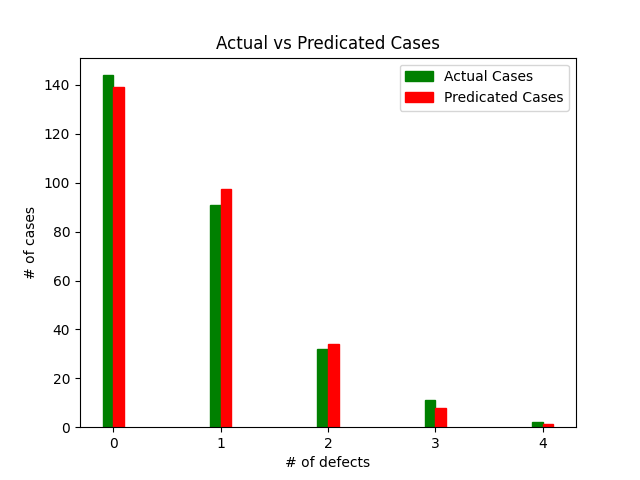
\includegraphics[width=\linewidth]{Figure_1.png}
        \caption{A barplot}
        \label{fig:barplot1}
    \end{figure}
	\newpage
	
	\subproblem{e} According to the barplot in (c), does the poisson distribution fit the data well? Compare the values of the actual cases and the values of the poisson predicted cases, and write your opinions about performance of the distribution.\\
	
	\begin{itemize}
	    \item We should compare the actual cases and predicted cases to determine whether poisson distribution fits the data well or not.
	    \item Number of actual cases: 280
	    \item Number of predicted cases: 279
	    \item As we can see, difference is not big here and we can see that poisson predicts this fairly well. When we evaluate in terms of performance, it can make very close prediction using Poisson distribution. Using the Poisson distribution can be efficient in terms of creating a predicted distribution data.
	\end{itemize}
	
	\subproblem{f} According to your estimations above, write your opinions considering your barplot and Table \ref{tab2}.Do you think that road transportation is dangerous for us? Whether yes or no, explain your reason.\\
	
	\begin{itemize}
	    \item We need to compare the numbers of real cases and predicted cases to decide whether road transportation is dangerous or not.
	    \item According to actual number of cases
	        \begin{itemize}
	            \item Total number of crash: 196
	            \item Total number of crash-free: 144
	            \item Crash rate = 196 / (144 + 196) = 0.576
	        \end{itemize}
	    \item According to predicted number of cases
	        \begin{itemize}
	            \item Total number of crash: 191
	            \item Total number of crash-free: 139
	            \item Crash rate = 191 / (139 + 191) = 0.578
	        \end{itemize}
        \item As we can see, we can say that the risk of crashes increased and we can say that road transportation is not safe.
	\end{itemize}
	
	\subproblem{g} Paste your code that you implemented for the subproblems above. Do not forget to write comments on your code.\\
	Example:\\
	\begin{itemize}
	
	\item The common code block for all subproblems\\
	\begin{lstlisting}[label={list:first},caption=The common code - Import modules and File operations]
    import scipy
    import matplotlib.pyplot as plot
    from scipy import stats
    import numpy as np
    
    DEFECT = 5
    
    def read():
        file = open("manufacturing_defects.txt", "r")
        data = []
    
        for line in file:
            row = []
            for i in line.split():
                if i.isdigit():
                    row.append(int(i))
            data.append(row)
        
        return data
    
    # counts defect for given defect_id
    def count_defects(data, defect_id):
        total = 0
    
        for i in data:
            total += i[1:].count(defect_id)
            
        return total
    
    data = read()
    num_of_company = len(data[0]) - 2 # -2 for first(row number) and second(year) column
    num_of_year = len(data)
    
    # print table
    table = print_table1(data)
    
    # find lambda
    mean = find_lambda(data, num_of_company, num_of_year)
    print(mean)
    
    # find estimations
    estimated_table = estimate(table, mean, num_of_company, num_of_year)
    print(estimated_table)
    
    # draw barplot
    barplot(table, estimated_table)
    \end{lstlisting}
	
	\item The code block for (a)\\
	\begin{lstlisting}[label={list:first},caption=The code block a - Compute the values in Table 1 and Print table]
	def print_table1(data):
        table = []
    
        for i in range(0, DEFECT):
            table.append(count_defects(data, i))
        
        print(table)
        return table
    \end{lstlisting}
	
	\item The code block for (b)\\
	\begin{lstlisting}[label={list:first},caption=The code block b - Compute Lambda]
	def find_lambda(data, num_of_company, num_of_year):
        total = 0
        
        for r in data:
            for i in range(len(r) - 2):
                total += r[i+2]
    
        return total / (num_of_company * num_of_year)
    \end{lstlisting}
	
	\item The code block for (c)\\
	\begin{lstlisting}[label={list:first},caption=The code block c - Compute the values in Table 2 and Print table]
    	def estimate(table, mean, num_of_company, num_of_year):
        predicated_cases_poisson = []
        total = 0
    
        for i in table:
            total += i
    
        for i in range(len(table)):
            predicated_cases_poisson.append(total * scipy.stats.poisson.pmf(i, mean))
    
        return predicated_cases_poisson
    \end{lstlisting}
	
	\item The code block for (d)\\
	\begin{lstlisting}[label={list:first},caption=The code block d - Draw the barplot]
	def barplot(table, estimated_table):
        w = 0.1
        
        real_plt = plot.bar(np.arange(DEFECT), table, w, label = "Actual Cases")
        est_plt = plot.bar(np.arange(DEFECT) + w, estimated_table, w, label = "Predicated Cases")
    
        for i in range(0, DEFECT):
            real_plt[i].set_color('g')
            est_plt[i].set_color('r')
    
        plot.title("Actual vs Predicated Cases")
        plot.xlabel("# of defects")
        plot.ylabel("# of cases")
        plot.xticks(np.arange(DEFECT) + w/2, [i for i in range(0, DEFECT)])
        plot.legend(loc = "best")
        plot.show()
    \end{lstlisting}
    \end{itemize}

\end{document} 